\section{Iterative PlasBin-flow binning method}\label{sec:pbf_iterbin}

In the following, a fragment can refer to both a pangenome fragment or a contig.
As an abuse of notation, we use in the whole section the set \Fragments{} to denote either the pan-assembly fragment set or the contig set.

The here presented Iterative PlasBin-flow binning method is an adaptation of the original PlasBin-flow method~\cite{manePlasBinflowFlowbasedMILP2023}.

The binning method consists in iteratively find the best bin by solving a flow-based combinatorial optimization problem on a network graph (defined in \Cref{sec:pbf_iterbin:network}).
Once a bin is found, we extract it from the network and continue the search until some criterion are not met.
For a given bin, each fragment is associated with a use of its coverage.
Extracting the bin from the network graph means decreasing the fragment coverages in the graph.
When the coverage a fragment in the network falls to zero, the fragment and its arcs are removed from graph.
\Cref{algo:pbf_iterbin} details the iterative binning process.

\begin{tcbalgo}{Iterative PlasBin-flow binning}{pbf_iterbin}
  \begin{algorithmic}[1]
    \Require{%
      A network graph \(N\) as in \Cref{definition:pbf_iterbin:network_graph}.
    }
    \Ensure{%
      Extract bins from the network graph.
    }
    \Function{extract\_bins}{\( N \)}
    \While{There are seeds in \(N\) and the previous model was feasible}
    \State{} \( find\_result \gets \Call{find\_best\_bin}{ N } \)
    \If{\( find\_result.\Call{feasibility\_message}{  } \) is a feasible message}
    \State{} Output \( find\_result.\Call{bin}{ } \)
    \State{} Extract the bin from the network graph \(N\) by updating the coverages.
    \EndIf{}
    \EndWhile{}
    \EndFunction{}
  \end{algorithmic}
\end{tcbalgo}

We propose three Mixed Integer Linear Programming (MILP) approaches to find the best bin (\( \Call{find\_best\_bin}{} \) subfunction, \Cref{sec:pbf_iterbin:decomp,sec:pbf_iterbin:binlab,sec:pbf_iterbin:once})
Each of them tries to answer to the PlasBin-flow discussion.

\begin{newfeatbox}
  Comparing to PlasBin-flow, we directly model the flow connectivity in the MILP models.
\end{newfeatbox}

The MILP models share subsets of variables and constraints we detail in \Cref{sec:pbf_iterbin:milp}.

%
% Common parts among the approaches
%
\subsection{The network graph}\label{sec:pbf_iterbin:network}

All the MILP flow-based approaches are built on the top of a flow network:

\begin{itemize}
  \item We add two vertices, \source{} and \sink{}, that are respectively the source and the sink vertices.
  \item The set \(\VSeeds{}\) contains the vertices associated with the seed contigs in \ContigSeeds{}.
    The source goes into each vertex in \(\VSeeds{}\), and each vertex in \(V_{\Contigs{}}\) goes into the sink.
\end{itemize}

\begin{notebox}
  We discuss in \zcref[S]{sec:pbf_iterbin:conclusions} the connection of the source to only the seeds.
\end{notebox}

\begin{definition}{Network graph}{pbf_iterbin:network_graph}
  Let \(N = (V, A, \source{}, \sink{}, \cov{\Contigs{}}, \gcscore{\Contigs{}}{K}, \plm{\Contigs{}})\) be the network graph, where:

  \begin{itemize}
    \item \( V = V_\Contigs{} \cup \Set*{\source{}, \sink{}} \) is the set of vertices with the source \(\source{}\) and the sink \(\sink{}\);
    \item \( A = A_\Links{} \cup \Set{(\source, v) \given v \in \VSeeds{}} \cup \Set{(v, \sink) \given v \in V} \) is the set of link-arcs augmented with the source-arcs and the sink-arcs;
    \item \( \cov{\Contigs{}} \colon \Contigs{} \to \Reals{}_{> 0} \) is the coverage function;
    \item \( \gcscore{\Contigs{}}{K} \colon \Contigs{} \times K \to [-1, 1] \) is the GC score function;
    \item \( \plm{\Contigs{}} \colon \Contigs{} \to [-1, 1] \) is the plasmidness function.
  \end{itemize}
\end{definition}


\subsection{Common Mixed Integer Linear Programming (MILP) objects}\label{sec:pbf_iterbin:milp}

\Cref{tab:pbf_iterbin:milp:variables} lists all the variables used in the MILP models.

\begin{table}
  \centering
  \tablecaptionof{MILP variable set}{%
    Each of the following variables participates in at least one of the MILP model.
    Some of them participate in all the model, others are necessary for only one model.
    For the ease of read, we categorize the variables in three categories.
    Each section describing a model precise which variables are participating for each category.
  }\label{tab:pbf_iterbin:milp:variables}

  \begin{longtable}{@{}llp{0.5\textwidth}@{}}
    \toprule
    \tabhtxt{Variable} & \tabhtxt{Application set} & \tabhtxt{Meaning} \\
    \midrule
    %
    \multicolumn{3}{@{}l@{}}{\tabhtxt{Decision variables}} \\
    \addlinespace
    \(x_v \in \Reals_{\geq 0}\) & \(\forall v \in V \setminus \Set*{s, t}\) & Denoting whether the vertex \(v\) is active or not. \\
    \addlinespace
    \(y_a \in \Set{0, 1}\) & \(\forall a \in A_\Links{}\) & Denoting whether the link-arc \(a\) is active or not. \\
    \addlinespace
    \(\frag{i} \in [0, 1] \) & \(\forall i \in \Fragments{}\) & Denoting whether fragment \(i\) is active or not. With the constraints it acts as a binary. \\
    \addlinespace
    \(GC_b \in \Set{0, 1}\) & \(\forall b \in K\) & Denoting whether the plasmid GC content is in the GC content interval \(b\) or not. \\
    \addlinespace
    \(\fraggc{i}{b} \in \Reals_{\geq 0}\) & \(\forall (i, b) \in \Fragments{} \times K\) & Denoting whether the fragment \(i\) is active and the plasmid GC content is in the interval \(b\) or not. With the constraints it acts as a binary. \\
    %
    \addlinespace
    \multicolumn{3}{@{}l@{}}{\tabhtxt{Flow variables}} \\
    \addlinespace
    \(f_a \in \Reals_{\geq 0}\) & \(\forall a \in A_\Links{}\) & Corresponding to the flow amount passing through the link-arc \(a\). \\
    \addlinespace
    \(F \in \Reals_{\geq 0}\) & & Corresponding to the overall flow. \\
    \addlinespace
    \(F_a \in \Reals_{\geq 0}\) & \(\forall a \in A_\Links{}\) & Playing the role of an intermediary variable to force the flow on each link-arc to be equal to the total flow. \\
    \addlinespace
    \(\inflowgc{i}{b} \in \Reals_{\geq 0}\) & \(\forall (i, b) \in \Fragments{} \times K\) & Corresponding to the flow amount passing through the fragment \(i\) when the plasmid GC content is in the interval \(b\). \\
    %
    \addlinespace
    \multicolumn{3}{@{}l@{}}{\tabhtxt{Connected component variables}} \\
    \addlinespace
    \(\alpha \in \Reals{}\) & & Is the number of \emph{oriented} fragments in the solution connected graph, plus the source and the sink. With the constraints it acts as a positive integer. \\
    \addlinespace
    \(\beta_a \in \Reals_{\leq 0}\) & \(\forall a \in A_\Links{}\) & Is strictly negative if the link-arc \(a\) participates in one of the solution subgraph's exploration tree. It acts as a negative integer, where the absolute value corresponds to the depth of the subtree defined by the successor. \\
    %
    \bottomrule
  \end{longtable}
\end{table}
Here we describe and categorize the set of constraints composing the different MILP models.
In what follow, we define either a fragment, a contig or an arc to be \enquote{active} if it participates in the solution, i.e.\ the flow passes through it.

\paragraph{Decision variables relationships}

A fragment is active if, and only if at least one of its extremity vertices is active:
\begin{align}
  x_v & \leq \frag{i} & \forall v \in V \setminus \Set*{s, t}, i = vfrag(v) \cstlabel{pbf_iterbin:milp:cst:dvar:active_extremity_implies_active_fragment} \\ % chktex 25
  \frag{i} & \leq x_u + x_v & \forall i \in \Fragments{}, \{u, v\} \in \EFrags{} \cstlabel{pbf_iterbin:milp:cst:dvar:active_fragment_implies_active_extremity} % chktex 25
\end{align}

The fragments involved in an active link-arc must also be active:
\begin{equation}
  y_{uv} \leq
  \begin{cases}
    x_v & \text{if \(u = s\)} \\
    x_u & \text{if \(v = t\)} \\
    \min\Set{x_u, x_v} & \text{otherwise}
  \end{cases} \quad \forall (u, v) \in A_\Links{} %
  \cstlabel{pbf_iterbin:milp:cst:dvar:active_link_arc_active_fragments} % chktex 25
\end{equation}

An active vertex implies at least one active link-arc incoming to it:
\begin{questionbox}
  Are these constraints necessary?
\end{questionbox}
\begin{equation}
  x_v \leq \sum_{(u, v) \in A_\Links{}} y_{u v} \quad \forall v \in V \setminus \Set{s, t} \cstlabel{pbf_iterbin:milp:cst:dvar:active_vertex_active_incoming_arcs} % chktex 25
\end{equation}

\paragraph{Flow constraints}

The flow through a link-arc \(a \in A_\Links{}\) is non-zero if \(a\) is active and cannot exceed its capacity:
\begin{align}
  f_{uv} \leq
  \begin{cases}
    \cov{j} y_{uv} & \text{if \(u = s\)} \\
    \cov{i} y_{uv} & \text{if \(v = t\)} \\
    \min\Set*{\cov{i}, \cov{j}} y_{uv} & \text{otherwise}
  \end{cases} &
  \begin{split}
    \forall (u, v) \in A_\Links{} \\
    i = vfrag(u) \\
    j = vfrag(v)
  \end{split} \cstlabel{pbf_iterbin:milp:cst:flow:arc_flow_at_most_coverage} % chktex 25
\end{align}

The cumulative flow through a fragment \(i \in \Fragments{}\) cannot exceed its read coverage:
\begin{equation}
  inflow(i) \leq \cov{i} \quad \forall i \in \Fragments{} \cstlabel{pbf_iterbin:milp:cst:flow:inflow_at_most_coverage} % chktex 25
\end{equation}
Where \(\displaystyle inflow(i) = \sum_{(u, i_t) \in A_\Links{}} f_{ui_t} + \sum_{(u, i_h) \in A_\Links{}} f_{ui_h}\) where \(i_t\) and \(i_h\) respectively stand for the tail and the head vertices of fragment \(i\).

The cumulative flow into a fragment \(i\) should be equal to the cumulative flow out of it. Same for the reverse \(i^-\):
\begin{align}
  \sum_{(u, i_t) \in A_\Links{}} f_{u i_t} & = \sum_{(i_h, w) \in A_\Links{}} f_{i_h w} & \forall i \in \Fragments{} \cstlabel{pbf_iterbin:milp:cst:flow:inflow_equals_outflow_forward} \\ % chktex 25
  \sum_{(u, i_h) \in A_\Links{}} f_{u i_h} & = \sum_{(i_t, w) \in A_\Links{}} f_{i_t w} & \forall i \in \Fragments{} \cstlabel{pbf_iterbin:milp:cst:flow:inflow_equals_outflow_reverse} % chktex 25
\end{align}

The total flow value \(F\) equals to the flow out of \(s\) and into \(t\):
\begin{align}
  F & = \sum_{(s, v) \in A_\Links{}} f_{sv} \cstlabel{pbf_iterbin:milp:cst:flow:total_flow_source} \\ % chktex 25
  F & = \sum_{(v, t) \in A_\Links{}} f_{vt} \cstlabel{pbf_iterbin:milp:cst:flow:total_flow_sink} % chktex 25
\end{align}

The total flow is strictly positive:
\begin{equation}
  F \geq \epsilon_F \quad \epsilon_F > 0 \cstlabel{pbf_iterbin:milp:cst:flow:total_flow_strictly_positive} % chktex 25
\end{equation}

An active link-arc has a flow at least \(F\).
\begin{align}
  F_a & \geq F - (1 - y_a) \max_{i \in \SeedFrags{}}\Set{\cov{i}} & \forall a \in A_\Links{} \cstlabel{pbf_iterbin:milp:cst:flow:arc_flow_at_least_total_flow_1} \\ % chktex 25
  F_a & \leq F & \forall a \in A_\Links{} \cstlabel{pbf_iterbin:milp:cst:flow:arc_flow_at_least_total_flow_2} \\ % chktex 25
  F_a & \leq f_a & \forall a \in A_\Links{} \cstlabel{pbf_iterbin:milp:cst:flow:arc_flow_at_least_total_flow_3} % chktex 25
\end{align}
\begin{infobox}
  These constraints do not force the arc flows to be a multiple of \(F\), see~\Cref{proposition:inflow_is_not_multiple_of_total_flow}.
\end{infobox}
\begin{missingproofbox}
  The above constraints minimize the number of out link-arcs for each fragment.
\end{missingproofbox}
\begin{questionbox}
  What is the meaning for a fragment to have a cumulative flow that is not a multiple of \(F\)?
  By keeping the flow real, can we smartly force the cumulative flow to be a multiple of \(F\)?
\end{questionbox}

\paragraph{Connected component constraints}

Exactly one link-arc outs of \(s\) is part of the solution (necessary to ensure the solution induced subgraph has only one connected component):
\begin{equation}
  \sum_{(s, v) \in A_\Links{}} y_{sv} = 1 \cstlabel{pbf_iterbin:milp:cst:ccomp:one_outgoing_arc_from_source} % chktex 25
\end{equation}

A positive flow implies the two incident vertices are in the component:
\begin{equation}
  1 - y_{uv} \geq
  \begin{cases}
    1 - x_v & \text{if \(u = s\)} \\
    x_u - 1 & \text{if \(v = t\)} \\
    x_u - x_v & \text{otherwise}
  \end{cases}
  \quad \forall (u, v) \in A_\Links{}
  \cstlabel{pbf_iterbin:milp:cst:ccomp:positive_flow_incident_vertices_in_component} % chktex 25
\end{equation}
\begin{questionbox}
  potentially redundant with \Cref{pbf_iterbin:milp:cst:dvar:active_vertex_active_incoming_arcs}
\end{questionbox}

The cumulative depth of the subtree in the exploration tree from the source equals at least the number of active vertices minus 1.
\begin{align}
  \alpha + \sum_{(s, w) \in A_\Links{}} \beta_{sw} \leq 1 \cstlabel{pbf_iterbin:milp:cst:ccomp:depth_of_tree_source} % chktex 25
\end{align}

Two incident arcs in the exploration tree are distanced by one.
\begin{align}
  \sum_{(v, w) \in A_\Links{}} \beta_{vw} - \sum_{(u, v) \in A_\Links{}} \beta_{uv} \leq 1 \quad \forall v \in V \setminus \Set*{s}
  \cstlabel{pbf_iterbin:milp:cst:ccomp:depth_of_tree_incident_arcs} % chktex 25
\end{align}

An arc participates in the exploration tree implies the arc is active.
\begin{align}
  \beta_a \geq - y_a |V| \quad \forall a \in A_\Links{}
  \cstlabel{pbf_iterbin:milp:cst:ccomp:tree_arc_active} % chktex 25
\end{align}

The number of active vertices equals \(\alpha{}\) (SAT constraint):
\begin{align}
  2 + \sum_{v \in V \setminus \Set*{s, t}} x_v = \alpha
  \cstlabel{pbf_iterbin:milp:cst:ccomp:number_of_active_vertices} % chktex 25
\end{align}

\paragraph{GC constraints}
%
The following constraints define the GC content labelling of a bin.

\phantom{text}

Only one GC content interval \(b \in K\) labels the bin:
\begin{equation}
  \sum_{b \in K} GC_b = 1
  \cstlabel{pbf_iterbin:milp:cst:gc:exactly_one_gc_content_interval} % chktex 25
\end{equation}

For each fragment \(i \in \Fragments{}\), for each GC content interval \(b \in K\), \(\fraggc{i}{b} = 1\) if and only if fragment \(i\) is active and the bin is labelled by the GC content interval \(b\):
\begin{align}
  \fraggc{i}{b} & \leq x_{i_t} + x_{i_h} & \forall (i, b) \in \Fragments{} \times K \cstlabel{pbf_iterbin:milp:cst:gc:active_fragment_gc_1} \\ % chktex 25
  \fraggc{i}{b} & \leq GC_b & \forall (i, b) \in \Fragments{} \times K \cstlabel{pbf_iterbin:milp:cst:gc:active_fragment_gc_2} \\ % chktex 25
  \fraggc{i}{b} & \geq x_{i_t} + GC_b - 1 & \forall (i, b) \in \Fragments{} \times K \cstlabel{pbf_iterbin:milp:cst:gc:active_fragment_gc_3} \\ % chktex 25
  \fraggc{i}{b} & \geq x_{i_h} + GC_b - 1 & \forall (i, b) \in \Fragments{} \times K \cstlabel{pbf_iterbin:milp:cst:gc:active_fragment_gc_4} % chktex 25
\end{align}

For each fragment \(i \in \Fragments{}\), for each GC content interval \(b \in K\), \(\inflowgc{i}{b}\) is the flow into fragment \(i\) when \(b\) is the chosen GC content interval:
\begin{align}
  \inflowgc{i}{b} & \leq \cov{i} \frag{i} *  & \forall (i, b) \in \Fragments{} \times K \cstlabel{pbf_iterbin:milp:cst:gc:inflowgc_1}  \\ % chktex 25
  \inflowgc{i}{b} & \leq \cov{i} GC_b & \forall (i, b) \in \Fragments{} \times K \cstlabel{pbf_iterbin:milp:cst:gc:inflowgc_2}  \\ % chktex 25
  \inflowgc{i}{b} & \geq inflow(i)  - (2 - \frag{i} - GC_b) \cov{i} & \forall (i, b) \in \Fragments{} \times K \cstlabel{pbf_iterbin:milp:cst:gc:inflowgc_3} % chktex 25
\end{align}

\paragraph{Plasmid constraints}

The cumulative fragment length is above a given threshold:
%
\begin{equation}
  \sum_{i \in \SeedFrags{}} |i| \geq L \quad L \geq 0 \cstlabel{pbf_iterbin:milp:cst:misc:min_cumulative_fragment_length} % chktex 25 chktex 35
\end{equation}
%
Typically, we choose \(L = 1000\).

%
% Approaches
%
\subsection{Approach \texttt{decomp}}\label{sec:pbf_iterbin:decomp}

\begin{newfeatbox}
  At the opposite of PlasBin-flow, we split each objective expression into different mono-objective functions that define different optimization problems.
\end{newfeatbox}
The \texttt{decomp} approach tackles the binning of the contigs with a coarse-to-fine-grain approach in four stages (each one refering to an optimization problem):

\begin{enumerate}[label=\roman*.]
  \item Find the maximum coverage flow (\MCF{} problem, \zcref[S]{sec:pbf_iterbin:decomp:mcf})
  \item Find the maximum GC score (\MGC{} problem, \zcref[S]{sec:pbf_iterbin:decomp:mgc})
  \item Find the maximum plasmidness score (\MPS{} problem, \zcref[S]{sec:pbf_iterbin:decomp:mps})
  \item Refine the solution (\MRCF{} problem, \zcref[S]{sec:pbf_iterbin:decomp:mrcf})
\end{enumerate}

\zcref[S]{algo:pbf_iterbin:decomp} summarizes the \texttt{decomp} approach.

\begin{tcbalgo}{\texttt{decomp} approach}{pbf_iterbin:decomp}
  \begin{algorithmic}[1]
    \Require{%
      A network graph \(N\) as in \zcref[S]{definition:pbf_iterbin:network_graph}.
    }
    \Ensure{%
      Extract the best bin from the network graph.
    }
    \Function{find\_best\_bin}{\( N \)}
    \State{} Init \MCF{} and solve it
    \If{\MCF{} is unfeasible}
    \State{} \Return{}unfeasible message
    \EndIf{}
    \State{} Init \MGC{} from \MCF{} result and solve it
    \If{\MGC{} is unfeasible}
    \State{} \Return{}unfeasible message
    \EndIf{}
    \State{} Init \MPS{} from \MGC{} result and solve it
    \If{\MPS{} is unfeasible}
    \State{} \Return{}unfeasible message
    \EndIf{}
    \State{} Init \MRCF{} from \MPS{} result and solve it
    \If{\MRCF{} is unfeasible}
    \State{} \Return{}unfeasible message
    \EndIf{}
    \State{} \Return{}\MRCF{} bin result (defined by the MILP solution variables induced subgraph)
    \EndFunction{}
  \end{algorithmic}
\end{tcbalgo}

Between each step, we fix the objective value of the previous step.
A final step refines the solution found in the \MPS{} step (\zcref[S]{sec:pbf_iterbin:decomp:mrcf}).

\subsubsection{The Maximum Coverage-likelihood Flow problem \MCF{}}\label{sec:pbf_iterbin:decomp:mcf}

The first binning stage consists in finding a flow maximizing the use of contig coverage.
We refer to this subproblem as the \enquote{Maximum Coverage-likelihood Flow} problem (\MCF{}).
As a coarse-grain strategy, it consists in finding a connected component explaining the coverages, large enough to contain all the contigs of the in-building solution bin.
Indeed, passing through a loop or a cycle will not change the flow value. Only maximizing the flow can lead to use a minimum of contigs.
To overcome this bias, we score the use of the contig coverages and maximize their total.
Below we describe the MILP model.

\begin{table}[h!]
  \centering
  \tablecaption{\MCF{} MILP constraints}{}\label{tab:decomp:mcf:cst}
  \begin{tabular}{@{}ll@{}}
    \toprule
    \tabhtxt{Category} & \tabhtxt{Constraints} \\
    \midrule
    Decision & \zcref[S]{%
      pbf_iterbin:milp:cst:dvar:active_vertex_implies_active_contig,%
      pbf_iterbin:milp:cst:dvar:active_contig_implies_active_vertex,%
      pbf_iterbin:milp:cst:dvar:active_arc_active_vertices,%
      pbf_iterbin:milp:cst:dvar:active_vertex_active_incoming_arcs%
    } \\
    Flow & \zcref[S]{%
      pbf_iterbin:milp:cst:flow:arc_flow_at_most_coverage,%
      pbf_iterbin:milp:cst:flow:inflow_at_most_coverage,%
      pbf_iterbin:milp:cst:flow:flow_conservation,%
      pbf_iterbin:milp:cst:flow:total_flow_strictly_positive,%
      pbf_iterbin:milp:cst:flow:total_flow_source,%
      pbf_iterbin:milp:cst:flow:total_flow_sink,%
      pbf_iterbin:milp:cst:flow:arc_flow_at_least_total_flow_1,%
      pbf_iterbin:milp:cst:flow:arc_flow_at_least_total_flow_2,%
      pbf_iterbin:milp:cst:flow:arc_flow_at_least_total_flow_3%
    } \\
    Connected component & \zcref[S]{%
      pbf_iterbin:milp:cst:ccomp:one_outgoing_arc_from_source,%
      pbf_iterbin:milp:cst:ccomp:positive_flow_incident_vertices_in_component,%
      pbf_iterbin:milp:cst:ccomp:depth_of_tree_source,%
      pbf_iterbin:milp:cst:ccomp:depth_of_tree_incident_arcs,%
      pbf_iterbin:milp:cst:ccomp:tree_arc_active,%
      pbf_iterbin:milp:cst:ccomp:number_of_active_vertices%
    } \\
    GC & --- \\
    Miscellaneous & \zcref[S]{%
      pbf_iterbin:milp:cst:misc:min_cumulative_contig_length%
    } \\
    \bottomrule
  \end{tabular}
\end{table}

\begin{definition}{\MCF{} MILP objective function}{pbf_iterbin:decomp:mcf:obj}
  \begin{newfeatbox}
    Here we maximize the coverage scores, not only the coverage flow.
  \end{newfeatbox}
  %
  The objective function aims to maximize the total coverage scores:
  \begin{Objective}
    \begin{equation}
      \max ~ CoverageScore
      \label{pbf_iterbin:decomp:mcf:obj:max_coverage_score} % chktex 25 % chktex 35
    \end{equation}
  \end{Objective}
  where
  \begin{align*}
    CoverageScore & = \sum_{i \in \Contigs{}} \fzeta{i} \parenth*{ inflow(i) - (\cov{i}\contig{i} - inflow(i)) } \\
    \fzeta{i} & = \frac{ |i| }{ \max_{j \in \Contigs{}} |j| }
  \end{align*}

  \begin{notebox}
    Before we had \(
      \displaystyle CoverageScore = %
      \sum_{i \in \Contigs{}} \parenth*{2 \frac{inflow(i)}{\cov{i}} - 1}
    \)
  \end{notebox}

  \begin{ideabox}
    You can get inspired from the future multi-flow ideas and define the coverage score to be:
    \[
      CoverageScore = \sum_{
        \substack{
          i \in \Contigs{} \\
          \plm{i} > 0
        }
      } |i| \parenth*{ inflow(i) - \cov{i} }
    \]
    where we focus on the use of positive plasmidness contigs, and try to minimize the penalty of not using their coverage.
    Multipliying by the contig length keep the things robust against the fragmentation of the sequences (good property for the assembly-consensus fragments).
  \end{ideabox}
\end{definition}
\subsubsection{The Maximum GC Score problem \MGC{}}\label{sec:pbf_iterbin:decomp:mgc}

The second binning stage consists in finding a flow maximizing the GC scores, by fixing the coverage score flow.
We refer to this subproblem as the \enquote{Maximum GC Score} problem (\MGC{}).
In the following we describe the MILP model.

\begin{table}[h!]
  \centering
  \tablecaption{\MGC{} MILP constraints}{}\label{tab:decomp:mgc:cst}
  \begin{tabular}{@{}ll@{}}
    \toprule
    \tabhtxt{Category} & \tabhtxt{Constraints} \\
    \midrule
    \multicolumn{2}{@{}l@{}}{Constraints in \zcref[S]{tab:decomp:mcf:cst}} \\
    \addlinespace
    GC & \zcref[S]{%
      pbf_iterbin:milp:cst:gc:exactly_one_gc_content_interval,%
      pbf_iterbin:milp:cst:gc:active_contig_gc_1,%
      pbf_iterbin:milp:cst:gc:active_contig_gc_2,%
      pbf_iterbin:milp:cst:gc:active_contig_gc_3,%
      pbf_iterbin:milp:cst:gc:active_contig_gc_4%
    } \\
    \MGC{} dedicated & \zcref[S]{pbf_iterbin:decomp:mgc:cst:fix_mcf_obj} \\
    \bottomrule
  \end{tabular}
\end{table}

In addition to the constraints in \zcref[S]{tab:decomp:mgc:cst}, we constraint the coverage score to be near to the optimal coverage score \(\Phi{}\) previously found in \MCF{}:
\begin{Constraint}
  \begin{equation}
    \Phi - (1 - \gamma_1) | \Phi | \leq CoverageScore \quad \gamma_1 \in (0.5, 1] % chktex 9
    \label{pbf_iterbin:decomp:mgc:cst:fix_mcf_obj} % chktex 25
  \end{equation}
\end{Constraint}

\begin{definition}{\MGC{} MILP objective function}{pbf_iterbin:decomp:mgc:obj}
  The objective function aims to maximize the GC score:
  \begin{Objective}
    \begin{equation}
      \max ~ GCScore
      \label{pbf_iterbin:decomp:mgc:obj:max_gc_probability_score} % chktex 25 % chktex 35
    \end{equation}
  \end{Objective}
  where \(
    \displaystyle GCScore = \sum_{\substack{
        i \in \Fragments{} \\
        b \in K
    }} \gcscore{i}{b} \fraggc{i}{b}%
  \).

  \begin{notebox}
    In the opposite of the other \texttt{decomp} models, in \MGC{} the GC score does not depend on the fragment coefficient \fzeta{i}.
  \end{notebox}
\end{definition}
\subsubsection{The Maximum Plasmidness Score problem \MPS{}}\label{sec:pbf_iterbin:decomp:mps}

The third binning stage consists in finding a flow maximizing the plasmidness scores, by fixing both the coverage flow and the GC score.
We refer to this subproblem as the \enquote{Maximum Plasmidness Score} problem (\MPS{}).
In the following we describe the MILP model.

\begin{table}[h!]
  \centering
  \tablecaption{\MPS{} MILP constraints}{}\label{tab:decomp:mps:cst}
  \begin{tabular}{@{}ll@{}}
    \toprule
    \tabhtxt{Category} & \tabhtxt{Constraints} \\
    \midrule
    \multicolumn{2}{@{}l@{}}{Constraints in \zcref[S]{tab:decomp:mgc:cst}} \\
    \addlinespace
    \MPS{} dedicated & \zcref[S]{pbf_iterbin:decomp:mps:cst:fix_mgc_obj} \\
    \bottomrule
  \end{tabular}
\end{table}

The total GC score value must be near to the total GC score best value \(\Psi{}\) previously found in \MGC{}:
\begin{Constraint}
  \begin{equation}
    \gamma_2 \Psi \leq GCScore \quad \gamma_2 \in (0.5, 1] % chktex 9
    \label{pbf_iterbin:decomp:mps:cst:fix_mgc_obj} % chktex 25
  \end{equation}
\end{Constraint}

\begin{definition}{\MPS{} MILP objective function}{pbf_iterbin:decomp:mps:obj}
  \begin{newfeatbox}
    While in the original PlasBin-flow method the plasmidness is positive, here the it either acts as a bonus or a penalty (\( \plm{i} \in [-1, 1] \)).
  \end{newfeatbox}
  %
  The objective function aims to maximize the plasmidness scores:
  \begin{Objective}
    \begin{equation}
      \max ~ PlasmidnessScore
      \label{pbf_iterbin:decomp:mps:obj:max_plasmidness_score} % chktex 25 % chktex 35
    \end{equation}
  \end{Objective}
  where \(\displaystyle PlasmidnessScore = \sum_{i \in \Fragments{}} \fzeta{i} \plm{i} \frag{i}\).
\end{definition}

\subsubsection{The Maximum Refined Coverage-likelihood Flow problem \MRCF{}}\label{sec:pbf_iterbin:decomp:mrcf}

The solution set \(S_\MPS{}\) for \MPS{} contains solutions with the same value of \(PlasmidnessScore\) and different values for \(CoverageFlow\) and \(GCScore\) because of \Cref{pbf_iterbin:decomp:mgc:cst:fix_mcf_obj,pbf_iterbin:decomp:mps:cst:fix_mgc_obj}.
The final refinement stage consists in fixing the value of \(PlasmidnessScore\) and finding the subset of \(S_\MPS{}\) maximizing first \(CoverageFlow\) and then \(GCScore\).
It results in a last MILP formulation \(\MRCF{}\):

\begin{table}[h!]
  \centering
  \tablecaption{\MRCF{} MILP constraints}{}\label{tab:decomp:mrcf:cst}
  \begin{tabular}{@{}ll@{}}
    \toprule
    \tabhtxt{Category} & \tabhtxt{Constraints} \\
    \midrule
    \multicolumn{2}{@{}l@{}}{Constraints in \Cref{tab:decomp:mps:cst}} \\
    \addlinespace
    \MRCF{} dedicated & \Cref{pbf_iterbin:decomp:mrcf:cst:fix_mps_obj} \\
    \bottomrule
  \end{tabular}
\end{table}

The plasmidness score must be equal to the plasmidness score \(P\) found in \MPS{}:
\begin{Constraint}
  \begin{equation}
    PlasmidnessScore = P
    \cstlabel{pbf_iterbin:decomp:mrcf:cst:fix_mps_obj} % chktex 25
  \end{equation}
\end{Constraint}

\begin{definition}{\MRCF{} MILP objective function}{pbf_iterbin:decomp:mrcf:obj}
  The objective function aims to maximize the coverage flow prior to the GC score:
  \begin{Objective}
    \begin{equation}
      \max ~ |\Fragments{}| CoverageFlow + GCScore
      \objlabel{pbf_iterbin:decomp:mrcf:max_coverage_and_gc_score} % chktex 25 % chktex 35
    \end{equation}
  \end{Objective}
\end{definition}


\subsection{Approach \texttt{binlab}}\label{sec:pbf_iterbin:binlab}

The \texttt{binlab} approach tackles the binning of the fragments with a coarse-to-fine-grain approach in three stages (each one refering to an optimization problem):
The ideas are quite similar to those in the \texttt{decomp} approach (\zcref[S]{sec:pbf_iterbin:decomp}), except that here we combine the use of the coverage and the plasmidness in one objective function.

\begin{enumerate}[label=\roman*.]
  \item Find the maximum binning score (\MBS{} problem, \zcref[S]{sec:pbf_iterbin:binlab:mbs})
  \item Find the maximum labelling score (\MLS{} problem, \zcref[S]{sec:pbf_iterbin:binlab:mls})
  \item Refine the solution (\MRBS{} problem, \zcref[S]{sec:pbf_iterbin:binlab:mrbs})
\end{enumerate}

\zcref[S]{algo:pbf_iterbin:binlab} summarizes the \texttt{binlab} approach.

\begin{tcbalgo}{\texttt{binlab} approach}{pbf_iterbin:binlab}
  \begin{algorithmic}[1]
    \Require{%
      A network graph \(N\) as in \zcref[S]{definition:pbf_iterbin:network_graph}.
    }
    \Ensure{%
      Extract the best bin from the network graph.
    }
    \Function{find\_best\_bin}{\( N \)}
    \State{} Init \MBS{} and solve it
    \If{\MBS{} is unfeasible}
    \State{} \Return{}unfeasible message
    \EndIf{}
    \State{} Init \MLS{} from \MBS{} result and solve it
    \If{\MLS{} is unfeasible}
    \State{} \Return{}unfeasible message
    \EndIf{}
    \State{} Init \MRBS{} from \MLS{} result and solve it
    \If{\MRBS{} is unfeasible}
    \State{} \Return{}unfeasible message
    \EndIf{}
    \State{} \Return{}\MRBS{} bin result (defined by the MILP solution variables induced subgraph)
    \EndFunction{}
  \end{algorithmic}
\end{tcbalgo}

Between each step, we fix the objective value of the previous step.
A final step refines the solution found in the \MLS{} step (\zcref[S]{sec:pbf_iterbin:binlab:mrbs}).

\subsubsection{The Maximum Binning Score problem \MBS{}}\label{sec:pbf_iterbin:binlab:mbs}

The first binning stage consists in finding a flow maximizing the use of fragment coverage and the plasmidness.
We refer to this subproblem as the \enquote{Maximum Binning Score} problem (\MBS{}).
As a coarse-grain strategy, it consists in finding a connected component explaining both the coverages and the plasmidness.
Below we describe the MILP model.

\begin{table}[h!]
  \centering
  \tablecaption{\MBS{} MILP constraints}{}\label{tab:binlab:mbs:cst}
  \begin{tabular}{@{}ll@{}}
    \toprule
    \tabhtxt{Category} & \tabhtxt{Constraints} \\
    \midrule
    Decision & \zcref[S]{%
      pbf_iterbin:milp:cst:dvar:active_vertex_implies_active_contig,%
      pbf_iterbin:milp:cst:dvar:active_contig_implies_active_vertex,%
      pbf_iterbin:milp:cst:dvar:active_arc_active_vertices,%
      pbf_iterbin:milp:cst:dvar:active_vertex_active_incoming_arcs%
    } \\
    Flow & \zcref[S]{%
      pbf_iterbin:milp:cst:flow:arc_flow_at_most_coverage,%
      pbf_iterbin:milp:cst:flow:inflow_at_most_coverage,%
      pbf_iterbin:milp:cst:flow:flow_conservation,%
      pbf_iterbin:milp:cst:flow:total_flow_source,%
      pbf_iterbin:milp:cst:flow:total_flow_sink,%
      pbf_iterbin:milp:cst:flow:total_flow_strictly_positive,%
      pbf_iterbin:milp:cst:flow:arc_flow_at_least_total_flow_1,%
      pbf_iterbin:milp:cst:flow:arc_flow_at_least_total_flow_2,%
      pbf_iterbin:milp:cst:flow:arc_flow_at_least_total_flow_3%
    } \\
    Connected component & \zcref[S]{%
      pbf_iterbin:milp:cst:ccomp:one_outgoing_arc_from_source,%
      pbf_iterbin:milp:cst:ccomp:positive_flow_incident_vertices_in_component,%
      pbf_iterbin:milp:cst:ccomp:depth_of_tree_source,%
      pbf_iterbin:milp:cst:ccomp:depth_of_tree_incident_arcs,%
      pbf_iterbin:milp:cst:ccomp:tree_arc_active,%
      pbf_iterbin:milp:cst:ccomp:number_of_active_vertices%
    } \\
    GC & --- \\
    Miscellaneous & \zcref[S]{%
      pbf_iterbin:milp:cst:misc:min_cumulative_contig_length%
    } \\
    \bottomrule
  \end{tabular}
\end{table}

\begin{definition}{\MBS{} MILP objective function}{pbf_iterbin:binlab:mbs:obj}
  The objective function aims to maximize the total coverage scores:
  \begin{Objective}
    \begin{equation}
      \max ~ BinningScore
      \label{pbf_iterbin:binlab:mbs:obj:max_coverage_score} % chktex 25 % chktex 35
    \end{equation}
  \end{Objective}
  where \(
    \displaystyle BinningScore = %
    \sum_{i \in \Fragments{}} \fzeta{i} \parenth[\big]{ inflow(i) - (\cov{i}\frag{i} - inflow(i)) + \plm{i} inflow(i)}
  \) and \( \displaystyle \fzeta{i} = \frac{ |i| }{ \max_{j \in \Fragments{}} |j| } \).

  \begin{ideabox}
    Perhaps we should use the coverage as a penalty and only on positive plasmidness, and replace \fzeta{} by the fragment length, i.e.:
    \[
      BinningScore =  \sum_{
        \substack{
          i \in \Fragments{} \\
          \plm{i} > 0
        }
      } |i| \parenth*{ inflow(i) - \cov{i} }
      + \sum_{i \in \Fragments{}} |i| \plm{i} inflow(i)
    \]
  \end{ideabox}
\end{definition}
\subsubsection{The Maximum Labelling Score problem \MLS{}}\label{sec:pbf_iterbin:binlab:mls}

The second binning stage consists in finding the best GC bin label, for a bin with a binning score lower bound.
We refer to this subproblem as the \enquote{Maximum Labelling Score} problem (\MLS{}).
In the following we describe the MILP model.

\begin{table}[!htbp]
  \centering
  \tablecaption{\MLS{} MILP constraints}{}\label{tab:binlab:mls:cst}
  \begin{tabular}{@{}ll@{}}
    \toprule
    \tabhtxt{Category} & \tabhtxt{Constraints} \\
    \midrule
    \multicolumn{2}{@{}l@{}}{Constraints in \zcref[S]{tab:binlab:mbs:cst}} \\
    \addlinespace
    GC & \zcref[S]{%
      pbf_iterbin:milp:cst:gc:exactly_one_gc_content_interval,%
      pbf_iterbin:milp:cst:gc:active_fragment_gc_1,%
      pbf_iterbin:milp:cst:gc:active_fragment_gc_2,%
      pbf_iterbin:milp:cst:gc:active_fragment_gc_3,%
      pbf_iterbin:milp:cst:gc:active_fragment_gc_4%
    } \\
    \MLS{} dedicated & \zcref[S]{pbf_iterbin:binlab:mls:cst:fix_mbs_obj} \\
    \bottomrule
  \end{tabular}
\end{table}

In addition to the constraints in \zcref[S]{tab:binlab:mls:cst}, we constraint the coverage score to be near to the optimal coverage score \(\Phi{}\) previously found in \MBS{}:
%
\begin{Constraint}
  \begin{equation}
    \Phi - (1 - \gamma_1) | \Phi | \leq BinningScore \quad \gamma_1 \in (0.5, 1] % chktex 9
    \cstlabel{pbf_iterbin:binlab:mls:cst:fix_mbs_obj} % chktex 25
  \end{equation}
\end{Constraint}

\begin{definition}{\MLS{} MILP objective function}{pbf_iterbin:binlab:mls:obj}

  The objective function aims to maximize the GC score:
  %
  \begin{Objective}
    \begin{equation}
      \max ~ LabellingScore
      \objlabel{pbf_iterbin:binlab:mls:obj:max_labelling_score} % chktex 25 % chktex 35
    \end{equation}
  \end{Objective}
  %
  where \(
    \displaystyle LabellingScore = \sum_{\substack{
        i \in \Fragments{} \\
        b \in K
    }} \gcscore{i}{b} \fraggc{i}{b}%
  \).

\end{definition}
\subsubsection{The Maximum Refining the \MLS{} solution}\label{sec:pbf_iterbin:binlab:mrbs}

The solution set \(S_\MLS{}\) for \MLS{} contains solutions with the same value of \(LabellingScore\) and different values for \(BinningScore\) because of \zcref[S]{pbf_iterbin:binlab:mls:cst:fix_mbs_obj}.
The final refinement stage consists in fixing the value of \(LabellingScore\) and finding the subset of \(S_\MLS{}\) maximizing \(BinningScore\).
It results in a last MILP formulation \(\MRBS{}\):

\begin{table}[h!]
  \centering
  \tablecaption{\MRBS{} MILP constraints}{}\label{tab:binlab:mrbs:cst}
  \begin{tabular}{@{}ll@{}}
    \toprule
    \tabhtxt{Category} & \tabhtxt{Constraints} \\
    \midrule
    \multicolumn{2}{@{}l@{}}{Constraints in \zcref[S]{tab:binlab:mls:cst}} \\
    \addlinespace
    \MRBS{} dedicated & \zcref[S]{pbf_iterbin:binlab:mrbs:cst:fix_mls_obj} \\
    \bottomrule
  \end{tabular}
\end{table}

The labelling score must be equal to the labelling score \(\Lambda{}\) found in \MLS{}:
\begin{Constraint}
  \begin{equation}
    LabellingScore = \Lambda
    \label{pbf_iterbin:binlab:mrbs:cst:fix_mls_obj} % chktex 25
  \end{equation}
\end{Constraint}

\begin{definition}{\MRBS{} MILP objective function}{pbf_iterbin:binlab:mrbs:obj}
  The objective function aims to maximize the binning score:
  \begin{Objective}
    \begin{equation}
      \max ~ BinningScore
      \label{pbf_iterbin:binlab:mrbs:obj:max_binning_score} % chktex 25 % chktex 35
    \end{equation}
  \end{Objective}
\end{definition}


\subsection{Approach \texttt{once}}\label{sec:pbf_iterbin:once}

The \texttt{once} approach tackles the binning of the fragments with only one optimization problem (\MGCLB{} problem, \zcref[S]{sec:pbf_iterbin:once:mgclb}) where the different bin properties are involved into only one objective function.
This approach is the nearer to the PlasBin-flow approach comparing to \texttt{decomp} and \texttt{binlab}.

\zcref[S]{algo:pbf_iterbin:once} summarizes the \texttt{once} approach.

\begin{tcbalgo}{\texttt{once} approach}{pbf_iterbin:once}
  \begin{algorithmic}[1]
    \Require{%
      A network graph \(N\) as in \zcref[S]{definition:pbf_iterbin:network_graph}.
    }
    \Ensure{%
      Extract the best bin from the network graph.
    }
    \Function{find\_best\_bin}{\( N \)}
    \State{} Init \MGCLB{} and solve it
    \If{\MGCLB{} is unfeasible}
    \State{} \Return{}unfeasible message
    \EndIf{}
    \State{} \Return{}\MGCLB{} bin result (defined by the MILP solution variables induced subgraph)
    \EndFunction{}
  \end{algorithmic}
\end{tcbalgo}

\subsubsection{The Maximum GC-Labelled Bin problem \MGCLB{}}\label{sec:pbf_iterbin:once:mgclb}

The first binning stage consists in finding a flow maximizing the use of fragment coverage and the plasmidness.
We refer to this subproblem as the \enquote{Maximum GC-Labelled Bin} problem (\MGCLB{}).
In the opposite of \texttt{decomp} and \texttt{binlab}, here we mix the GC scores with the other bin properties.
In order  balance the weight of the different semantic terms, we multiply by the incoming flow.
The more a fragment participates in terms of its coverage in the bin, the more its properties are amplified.
The length of the fragments also enable to balance the usage of the fragments in the bin.
It is also robust to the fragmentation (linear decomposition).
Below we describe the MILP model.

\begin{table}[h!]
  \centering
  \tablecaption{\MGCLB{} MILP constraints}{%
    What is new here comparing to the two previous approaches is we need to define variables \(\inflowgc{i}{b}\) for all fragments \(i \in \Fragments{}\) and GC content interval \(b \in K\).
    Also, we do not need to define the \(\fraggc{\Fragments}{K}\) binary variables.
  }\label{tab:once:mgclb:cst}
  \begin{tabular}{@{}ll@{}}
    \toprule
    \tabhtxt{Category} & \tabhtxt{Constraints} \\
    \midrule
    Decision & \zcref[S]{%
      pbf_iterbin:milp:cst:dvar:active_vertex_implies_active_contig,%
      pbf_iterbin:milp:cst:dvar:active_contig_implies_active_vertex,%
      pbf_iterbin:milp:cst:dvar:active_arc_active_vertices,%
      pbf_iterbin:milp:cst:dvar:active_vertex_active_incoming_arcs%
    } \\
    Flow & \zcref[S]{%
      pbf_iterbin:milp:cst:flow:arc_flow_at_most_coverage,%
      pbf_iterbin:milp:cst:flow:inflow_at_most_coverage,%
      pbf_iterbin:milp:cst:flow:flow_conservation,%
      pbf_iterbin:milp:cst:flow:total_flow_source,%
      pbf_iterbin:milp:cst:flow:total_flow_sink,%
      pbf_iterbin:milp:cst:flow:total_flow_strictly_positive,%
      pbf_iterbin:milp:cst:flow:arc_flow_at_least_total_flow_1,%
      pbf_iterbin:milp:cst:flow:arc_flow_at_least_total_flow_2,%
      pbf_iterbin:milp:cst:flow:arc_flow_at_least_total_flow_3%
    } \\
    Connected component & \zcref[S]{%
      pbf_iterbin:milp:cst:ccomp:one_outgoing_arc_from_source,%
      pbf_iterbin:milp:cst:ccomp:positive_flow_incident_vertices_in_component,%
      pbf_iterbin:milp:cst:ccomp:depth_of_tree_source,%
      pbf_iterbin:milp:cst:ccomp:depth_of_tree_incident_arcs,%
      pbf_iterbin:milp:cst:ccomp:tree_arc_active,%
      pbf_iterbin:milp:cst:ccomp:number_of_active_vertices%
    } \\
    GC & \zcref[S]{%
      pbf_iterbin:milp:cst:gc:exactly_one_gc_content_interval,%
      pbf_iterbin:milp:cst:gc:inflowgc_1,%
      pbf_iterbin:milp:cst:gc:inflowgc_2,%
      pbf_iterbin:milp:cst:gc:inflowgc_3%
    } \\
    Miscellaneous & \zcref[S]{%
      pbf_iterbin:milp:cst:misc:min_cumulative_contig_length%
    } \\
    \bottomrule
  \end{tabular}
\end{table}

\begin{definition}{\MGCLB{} MILP objective function}{pbf_iterbin:once:mgclb:obj}
  The objective function aims to maximize the total coverage scores:
  \begin{Objective}
    \begin{equation}
      \max ~ CoveragePenaly + PlasmidnessScore + GCScore
      \label{pbf_iterbin:once:mgclb:obj:max_coverage_score} % chktex 25 % chktex 35
    \end{equation}
  \end{Objective}
  where:
  \begin{align*}
    CoveragePenaly &= %
    \sum_{i \in \Fragments{}} |i| \parenth*{ inflow(i) - \cov{i}\frag{i} } \\
    PlasmidnessScore &= %
    \sum_{i \in \Fragments{}} |i| \plm{i} inflow(i) \\
    GCScore &= %
    \sum_{\substack{
        i \in \Fragments{} \\
        b \in K
    }} |i| \gcscore{i}{b} \inflowgc{i}{b}
  \end{align*}

  \begin{ideabox}
    Perhaps we should use the penalty coverage on only fragments with positive plasmidness.
  \end{ideabox}
\end{definition}

%
% Conclusions
%
\subsection{Results and conclusions}\label{sec:pbf_iterbin:conclusions}

I tested the three approaches on 12 samples from 4 different bacteria read samples, assembled by Unicycler, and where the contigs of size less than 100 were replaced by links in the assembly graph.
This subset covers several scenarios:

\begin{itemize}
  \item Some instances have connected components with only one contig looping on itself --- corresponding to circular plasmids (with, or without seeds);
  \item Some plasmids correspond to subgraph where a circular topology can be found (with or without seeds);
  \item Some plasmids correspond to subgraph where it is not possible to find a circular topology (missing links, with or without seeds).
\end{itemize}

\begin{warningbox}
  The Unicycler assembly graphs were malformed: some of the link definition were reversed (not in the sense of the reverse symmetry equivalence of defining one link and its reverse).
  This created many tips in the graph and denatured the cyclicity of subgraph corresponding to circular plasmids.
  However, many observations remain correct.
\end{warningbox}

\paragraph{The iterative binning process over-optimizes the first bin scores}
The first bin was mainly often the most difficult one to obtain.
In any case, the first bin is the largest one.
Each approach in the iterative binning process over-optimizes the scores of the first bin.
One of the main consequence is the first bin contains too much contigs, leading to remove contigs needed to get the next plasmids.
Thus, the next remain of plasmids are dispatched in several bins.
\Cref{fig:pbf_iterbin:merge_trap} provides a simple instance for which the iterative approach over-optimizes the first bin by merging several plasmids.
It also shows that additional bin topological constraint on the circularity does not solve the problem in the context of iterative binning.

\begin{figure}
  \centering
  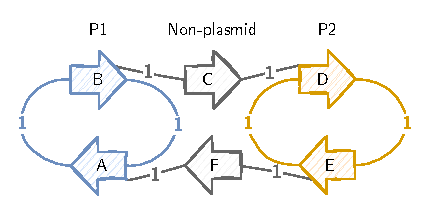
\includegraphics{pbf_iterbin/img/pbf_iterbin-merge_trap.pdf}
  \figurecaption{The first bin is more likely to be a merge of several plasmids.}{%
    Fragments of plasmid \(\mathsf{P1}\) (\(\mathsf{A}\) and \(\mathsf{B}\)) and those of plasmid \(\mathsf{P2}\) (\(\mathsf{D}\) and \(\mathsf{E}\)) are connected through two non-plasmid fragments (\(\mathsf{C}\) and \(\mathsf{F}\)).
    The number on links are their capacity in the network graph.
    As instance, let assume that the coverages of all the fragments equal \(1\), all the lengths equal \(100\), the plasmidness to be perfect (i.e.\ equal to \(1\) for plasmids' fragments and \(0\) for the others) as well as the seed set (containing only plasmids' fragments).
    Also, we consider only one GC content interval such that all the GC scores equal \(1\).
    The best bin is a merge of plasmid \(\mathsf{P1}\) and \(\mathsf{P2}\), corresponding to the flow \(\mathsf{S} \to \mathsf{A_f} \to \mathsf{B_f} \to \mathsf{C_f} \to \mathsf{D_f} \to \mathsf{E_f} \to \mathsf{T}\) (with score in \Cref{pbf_iterbin:once:mgclb:obj:max_coverage_score} equals to \(900\), for a total flow of \(1\)).
    Unfortunately, forcing the model to find a flow which can correspond to a circuit (circular bin) does not solve the problem here (the best bin remains a merge of \(\mathsf{P1}\) and \(\mathsf{P2}\), containing all the fragments).
  }\label{fig:pbf_iterbin:merge_trap}
\end{figure}

\paragraph{The MILP solving time is too long for a poor quality}
As described above, finding the first bin is the most difficult one to obtain, especially about time performance.
The MIP gap is sometimes really near to 0\% (optimal criterion) but slightly decreases.
Finding a MIP gap threshold for which we accept the feasible solution is not as easy, and no satisfying threshold was found (no more than 5\%).

\paragraph{Linearly handling the GC content of each contig seems to not be relevant}
Involving the GC content for plasmid binning through different non-intersecting intervals does not seem to help.
Here, we combine linearly the GC content of each contig through a positive flow passes.
While the flow can describe walks, we are not able (MILP limitation) to update the GC content of the extended sequence, and thus getting the true GC score for a given interval.
Note that GplasCC is updating the plasmid statistics each time it extends a walk (reconsider the whole extended sequence).

\paragraph{Connecting the source only to the seeds can split plasmid into several bins}
All the three approaches are based on a network graph where the source only connects the seeds.
When a link miss to satisfy the plasmid circularity, the recall and the precision become highly sensitive to the position of the seeds in the plasmid corresponding subgraph walk.
\Cref{fig:pbf_iterbin:seed_position_robustness} illustrates this issue.
As in \Cref{subfig:pbf_iterbin:middle_seed_splits_partially_circular_plasmid}, the recall decreases because we miss a fragment before the seed in the walk.
If this (positive plasmidness) fragment can be reached from another seed of another plasmid, it would appear in a different and wrong bin because it would enable the improvement of the objective function value at the time of this future bin search, resulting in a loss of precision.

\begin{figure}
  \centering
  \begin{subfigure}{0.45\linewidth}
    \centering
    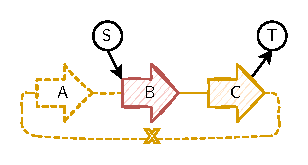
\includegraphics[width=\linewidth]{pbf_iterbin/img/pbf_iterbin-middle_seed_splits_partially_circular_plasmid.pdf}
    \caption{Seed splitting a partially circular bin}\label{subfig:pbf_iterbin:middle_seed_splits_partially_circular_plasmid}
  \end{subfigure}
  \hfill
  \begin{subfigure}{0.45\linewidth}
    \centering
    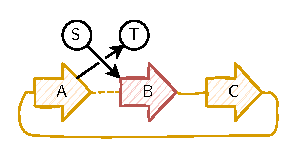
\includegraphics[width=\linewidth]{pbf_iterbin/img/pbf_iterbin-true_circularity_seed_robust.pdf}
    \caption{The circularity can avoid missing a fragment}\label{subfig:pbf_iterbin:true_circularity_seed_robust}
  \end{subfigure}
  \hfill
  \begin{subfigure}{\linewidth}
    \centering
    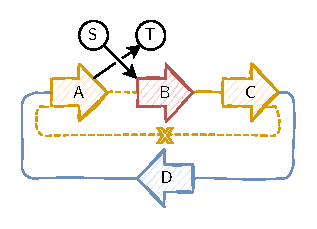
\includegraphics[width=0.45\linewidth]{pbf_iterbin/img/pbf_iterbin-circularity_artefact.pdf}
    \caption{A circularity artefact}\label{subfig:pbf_iterbin:circularity_artefact}
  \end{subfigure}
  \figurecaption{The search for a bin is highly sensitive to the seed position in a partially circular plasmid context}{%
    In each subfigure, fragments \(\mathsf{A}\), \(\mathsf{B}\) and \(\mathsf{C}\) and their links belong to the same plasmid.
    For all this fragments, we assume to be in an almost-perfect case: they all have the same coverage and the same best GC interval, and the plasmidness equals.
    However, the seed set only contains the red fragment \(\mathsf{B}\).
    A cross means the link does not exist while it should to satisfy the circularity of the plasmid.
    A dashed fragment or link is not active.
    %
    \Subref{subfig:pbf_iterbin:middle_seed_splits_partially_circular_plasmid}
    %
    The crossed link is missing so that it is not possible to complete the plasmid circularity.
    Since the seed is now in the middle of the path, and as according to the network definition the source only connects to the seed fragments, then the best bin misses the fragment \(\mathsf{A}\).
    %
    \Subref{subfig:pbf_iterbin:true_circularity_seed_robust}
    %
    If now the link is not missing, it is possible to retrieve \(\mathsf{A}\) by positioning it at the end of the walk, and outgoing after it to the sink (which connects to all the fragments).
    %
    \Subref{subfig:pbf_iterbin:circularity_artefact}
    %
    Suppose now we face the same situation as in \subref{subfig:pbf_iterbin:middle_seed_splits_partially_circular_plasmid} but fragment \(\mathsf{D}\) --- which does not belong to the orange plasmid, enables the circularity.
    Under some circumstances, passing through this fragment can improve the objective function value because it enables to retrieve \(\mathsf{A}\).
    If \(b \in K\) is the GC content interval associated with the orange plasmid, then it is sufficient to have \( inflow(\mathsf{D}) (1 + \plm{\mathsf{D}} + \gcscore{\mathsf{D}}{b}) - \cov{\mathsf{D}} \geq 0\) to retrieve \(\mathsf{A}\) through \(\mathsf{D}\).

  }\label{fig:pbf_iterbin:seed_position_robustness}
\end{figure}

\paragraph{The positive flow constraint raises the complexity in a circular plasmid context}

As in PlasBin-flow, we require the flow on each arc to be at least equal to the total flow (i.e.\ the sum of the flow outgoing from the source).
The total flow thus conveniently encodes the multiplicity of a unique region in the genome the bin represents.
However, it increases the number of equivalent solutions in a circular plasmid context.
\Cref{fig:pbf_iterbin:implicit_circularity} illustrates this phenomenon.
Removing this constraint can improve the performances.
Also, it is the occasion to better model the circularity.

\begin{figure}
  \centering
  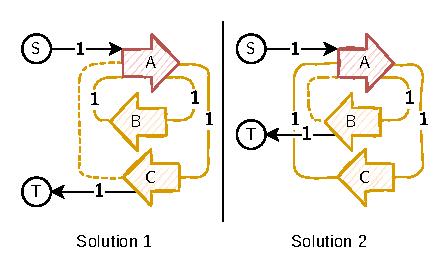
\includegraphics{pbf_iterbin/img/pbf_iterbin-implicit_circularity.pdf}
  \figurecaption{The circularity multiplies the number of equivalent solutions}{%
    Suppose we have a plasmid with three fragments, where \(\mathsf{A}\) is the seed and also a repeated sequence in the plasmid genome, such that its coverage is twice the ones of \(\mathsf{B}\) and \(\mathsf{C}\).
    Dashed links are not active.
    Active links are associated with a flow number.
    Because we force the flow on the arcs to equal at least the total flow, in a circular context the best solutions consist in replacing one of the link that connects a unique region by the source-link and the sink-link, which emulate the circularity.
    This results in a set of equivalent solutions, and then to an increase of the branch-and-bound time consumption.
  }\label{fig:pbf_iterbin:implicit_circularity}
\end{figure}